\myChapter{Experiments}
\label{chap:Experiments}

In this chapter, various experiments and their corresponding results will be showcased, highlighting the inference speed and image quality assessment. Basic PyTorch implementations of UNet and SRUNet will be used, as well as their compiled counterparts with TensorRT, allowing for different precisions of weights/activations, namely FP32, FP16, and INT8.

\section{Quantitative Results}
\label{sec:quantitative-results}

\Cref{tab:perceptual-metrics,tab:traditional-metrics} present the performance of UNet and SRUNet models, as well as their TensorRT-optimized versions (FP32, FP16, INT8), on perceptual and traditional metrics over 60 test frames.

The perceptual metrics used for evaluation are LPIPS, DISTS, and BRISQUE. Lower values of these metrics indicate better image quality. \Cref{tab:perceptual-metrics} shows that the UNet model and its optimized versions have similar performance in LPIPS and DISTS, with the INT8 version showing a slight decrease in these metrics. Both UNet and SRUNet models slightly improve in terms of the BRISQUE score when optimized to INT8.

SSIM, MS-SSIM, and PSNR are the non-perceptual metrics used for evaluation. For these metrics, higher values indicate better image quality. In \cref{tab:traditional-metrics}, both UNet and SRUNet models show similar performance across all precisions in SSIM and MS-SSIM. The UNet model has a slightly higher PSNR value than the SRUNet model, and the INT8-optimized versions of both models have marginally lower PSNR values compared to their FP32 and FP16 counterparts.

\Cref{tab:vmaf} shows VMAF scores (see \cref{sec:video-quality-metrics}) for both UNet and SRUNet models, and their optimized versions using a test video of 2-minute length. The harmonic mean is shown because if there were outliers (i.e., frames for which the score is lower than average by more than a certain number of standard deviations) the score would decrease substantially more than the traditional average.

In general, the differences in performance between the plain models and their optimized versions are relatively small for both perceptual and traditional metrics.

Execution times for both UNet and SRUNet, along with their TensorRT-optimized versions (FP32, FP16, INT8), are shown in \cref{tab:timings}. Both UNet and SRUNet models demonstrate reduced evaluation times across all precisions. The INT8-optimized version exhibit the fastest evaluation times for both models, followed by FP16 and FP32 versions.
Moreover, the SRUNet model consistently outperforms the UNet model for all precisions, and the relatively small standard deviations indicate consistent performance over the 300 runs.
For a visual representation, see \cref{fig:timings}.

The INT8-optimized UNet and SRUNet models achieve 2.38X and 2.26X speedup compared to their original implementations, respectively. Furthermore, memory consumption was reduced up to 63.3\% for the UNet (from 30MB to 11MB) and up to 53.8\% (from 2.6MB to 1.2MB) for the SRUNet using the INT8 versions.

\begin{table*}[t]
\begin{tabular}{llll}
\toprule
{} & LPIPS $\downarrow$ & DISTS $\downarrow$ & BRISQUE $\downarrow$ \\
\midrule
UNet        &  \textbf{0.2897 ± 0.0138} &  \textbf{0.1222 ± 0.0067} &  31.1372 ± 1.1690 \\
UNet-FP32   &  \textbf{0.2897 ± 0.0138} &  \textbf{0.1222 ± 0.0067} &  31.1373 ± 1.1684 \\
UNet-FP16   &  0.2898 ± 0.0138 &  0.1223 ± 0.0067 &  31.1383 ± 1.1691 \\
UNet-INT8   &  0.3041 ± 0.0137 &  0.1283 ± 0.0066 &  \textbf{29.6849 ± 1.0138} \\
\midrule
SRUNet      &  0.3111 ± 0.0151 &  \textbf{0.1717 ± 0.0047} &  27.3738 ± 3.5705 \\
SRUNet-FP32 &  0.3111 ± 0.0151 &  \textbf{0.1717 ± 0.0047} &  27.3736 ± 3.5697 \\
SRUNet-FP16 &  0.3111 ± 0.0151 &  \textbf{0.1717 ± 0.0047} &  27.3790 ± 3.5739 \\
SRUNet-INT8 &  \textbf{0.3068 ± 0.0137} &  0.1722 ± 0.0044 &  \textbf{26.1546 ± 3.2273} \\
\bottomrule
\end{tabular}
\caption{Evaluations on perceptual metrics on 60 test frames (mean $\pm$ standard deviation).}
\label{tab:perceptual-metrics}
\end{table*}

\begin{table*}[t]
\begin{tabular}{llll}
\toprule
{} & SSIM $\uparrow$ & MS-SSIM $\uparrow$ & PSNR $\uparrow$ \\
\midrule
UNet        &  \textbf{0.8952 ± 0.0084} &  \textbf{0.8517 ± 0.0067} &  \textbf{21.6506 ± 0.1269} \\
UNet-FP32   &  \textbf{0.8952 ± 0.0084} &  \textbf{0.8517 ± 0.0067} &  \textbf{21.6506 ± 0.1269} \\
UNet-FP16   &  \textbf{0.8952 ± 0.0084} &  \textbf{0.8517 ± 0.0067} &  \textbf{21.6506 ± 0.1269} \\
UNet-INT8   &  0.8941 ± 0.0084 &  0.8508 ± 0.0067 &  21.6388 ± 0.1286 \\
\midrule
SRUNet      &  \textbf{0.8894 ± 0.0084} &  \textbf{0.8457 ± 0.0062} &  21.3670 ± 0.1248 \\
SRUNet-FP32 &  \textbf{0.8894 ± 0.0084} &  \textbf{0.8457 ± 0.0062} &  21.3670 ± 0.1248 \\
SRUNet-FP16 &  \textbf{0.8894 ± 0.0084} &  \textbf{0.8457 ± 0.0062} &  \textbf{21.3671 ± 0.1248} \\
SRUNet-INT8 &  0.8882 ± 0.0084 &  \textbf{0.8442 ± 0.0062} &  21.3320 ± 0.1224 \\
\bottomrule
\end{tabular}
\caption{Evaluations on traditional metrics on 60 test frames (mean $\pm$ standard deviation).}
\label{tab:traditional-metrics}
\end{table*}

\begin{table*}[t]
\begin{tabular}{lrr}
\toprule
{} &       VMAF (mean) $\uparrow$ &  VMAF (harmonic mean) $\uparrow$ \\
\midrule
UNet        &  47.71 &      47.20 \\
UNet-FP32   &  \textbf{47.72} &      \textbf{47.21} \\
UNet-FP16   &  47.71 &      47.20 \\
UNet-INT8   &  47.47 &      46.96 \\
\midrule
SRUNet      &  \textbf{47.20} &      \textbf{46.65} \\
SRUNet-FP32 &  47.19 &      46.64 \\
SRUNet-FP16 &  47.19 &      \textbf{46.65} \\
SRUNet-INT8 &  47.18 &      46.64 \\
\bottomrule
\end{tabular}
\caption{VMAF scores on a 120-second-test video.}
\label{tab:vmaf}
\end{table*}

\begin{figure*}[ht]
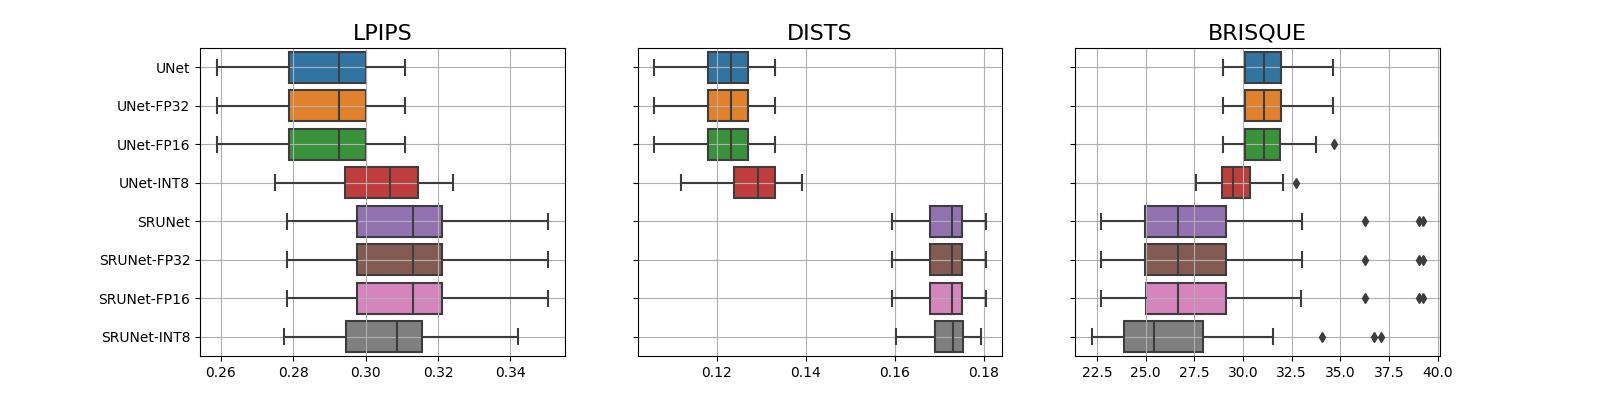
\includegraphics[width=1.0\textwidth]{static/boxplots_perceptual_metrics.jpg}
\caption{Box-plots of perceptual metrics on 60 test frames (the lower, the better).}
\label{fig:perceptual-metrics}
\end{figure*}

\begin{figure*}[ht]
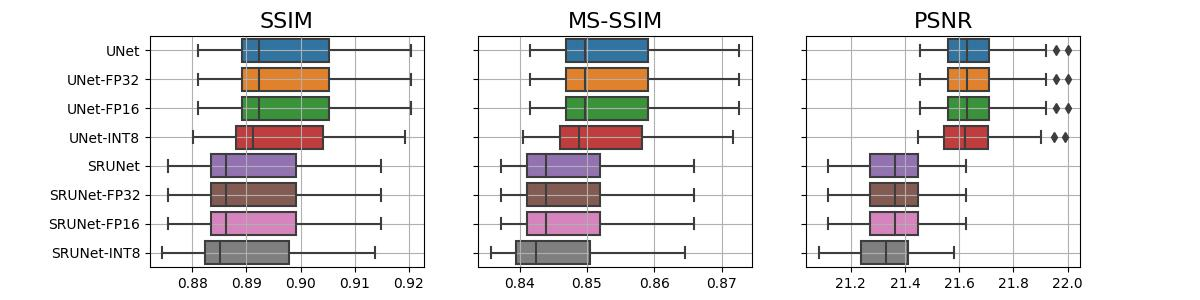
\includegraphics[width=1.0\textwidth]{static/boxplots_traditional_metrics.jpg}
\caption{Box-plots of traditional metrics on 60 test frames (the higher, the better).}
\label{fig:traditional-metrics}
\end{figure*}

\begin{table*}[t]
\begin{tabular}{lll}
\toprule
{} &      times [s] $\downarrow$ & speedup $\uparrow$ \\
\midrule
UNet        &  0.0348 ± 0.0004 & {} \\
UNet-FP32   &  0.0279 ± 0.0004 & 1.247X \\
UNet-FP16   &  0.0279 ± 0.0004 & 1.247X \\
UNet-INT8   &  \textbf{0.0146 ± 0.0006} & \textbf{2.38X} \\
\midrule
SRUNet      &  0.0123 ± 0.0001 & {} \\
SRUNet-FP32 &  0.0087 ± 0.0005 & 1.41X \\
SRUNet-FP16 &  0.0087 ± 0.0004 & 1.41X \\
SRUNet-INT8 &  \textbf{0.0054 ± 0.0006} & \textbf{2.27X} \\
\bottomrule
\end{tabular}
\caption{Evaluation times over 300 runs (mean $\pm$ standard deviation).}
\label{tab:timings}
\end{table*}

\begin{figure*}[ht]
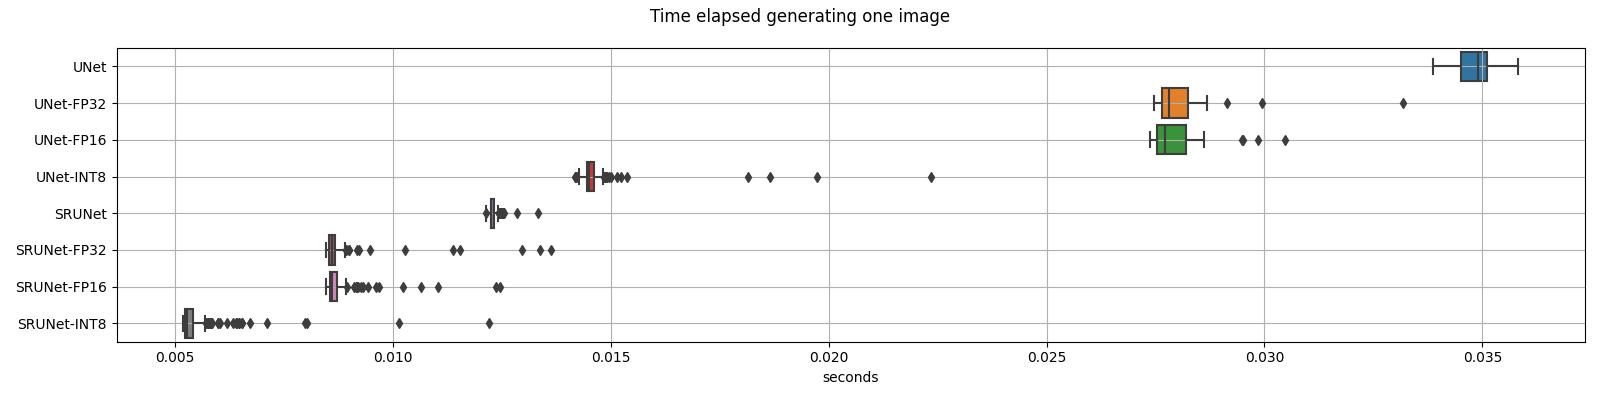
\includegraphics[width=1.0\textwidth]{static/boxplots_timings.jpg}
\caption{Average times elapsed in seconds for generating one image using different versions of UNet and SRUNet implementations.}
\label{fig:timings}
\end{figure*}

% \begin{table*}[t]
% \begin{tabular}{ll}
% \toprule
% {} &      size \\
% \midrule
% UNet        & 30MB \\
% % UNet-FP32   & 71MB \\
% % UNet-FP16   & 71MB \\
% UNet-INT8   & 11MB \\
% \midrule
% SRUNet      & 2.6MB \\
% % SRUNet-FP32 & 6.3MB \\
% % SRUNet-FP16 & 6.3MB \\
% SRUNet-INT8 & 1.2MB \\
% \bottomrule
% \end{tabular}
% \caption{Memory consumption of UNet and SRUNet model weights, as well as their compiled versions using TensorRT with precisions INT8. It is noteworthy that the compiled INT8 version also stores the full model graph, its weights, and the calibrated quantization maps.}
% \label{tab:memory-consumption}
% \end{table*}

\clearpage

\section{Qualitative Results}
\label{sec:qualitative-results}

\Cref{fig:qualitative-unet} and \cref{fig:qualitative-srunet} show no decrease in the quality of a generated image among plain and compiled versions of the UNet and SRUNet models. The evaluations were done on a 96$\times$96 patch from a frame of a test video.

\begin{figure*}[ht]
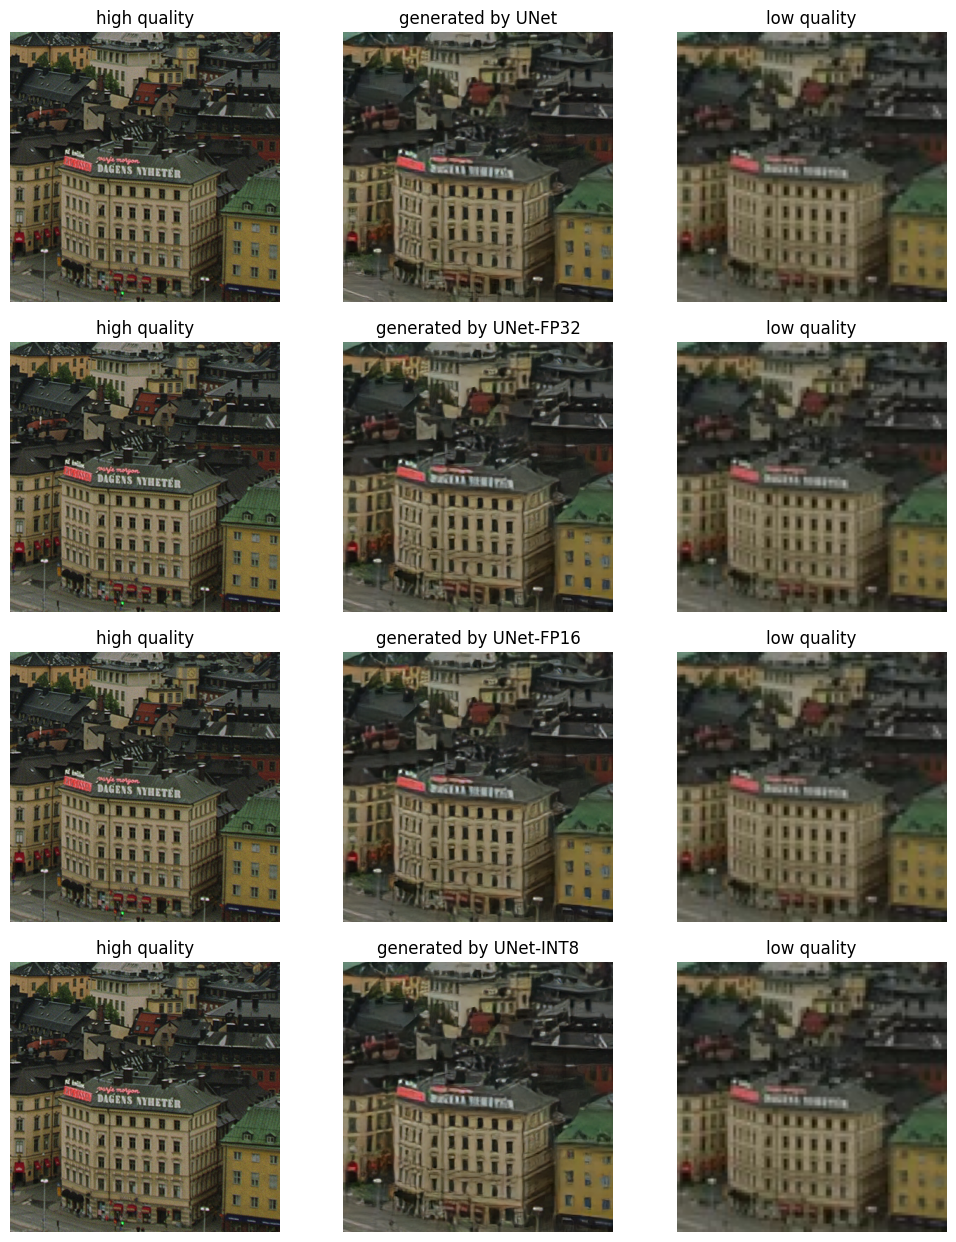
\includegraphics[width=0.8\textwidth]{static/unet_qualitative_results.png}
\caption{Qualitative results for each variation of the UNet model on a test patch.}
\label{fig:qualitative-unet}
\end{figure*}

\begin{figure*}[ht]
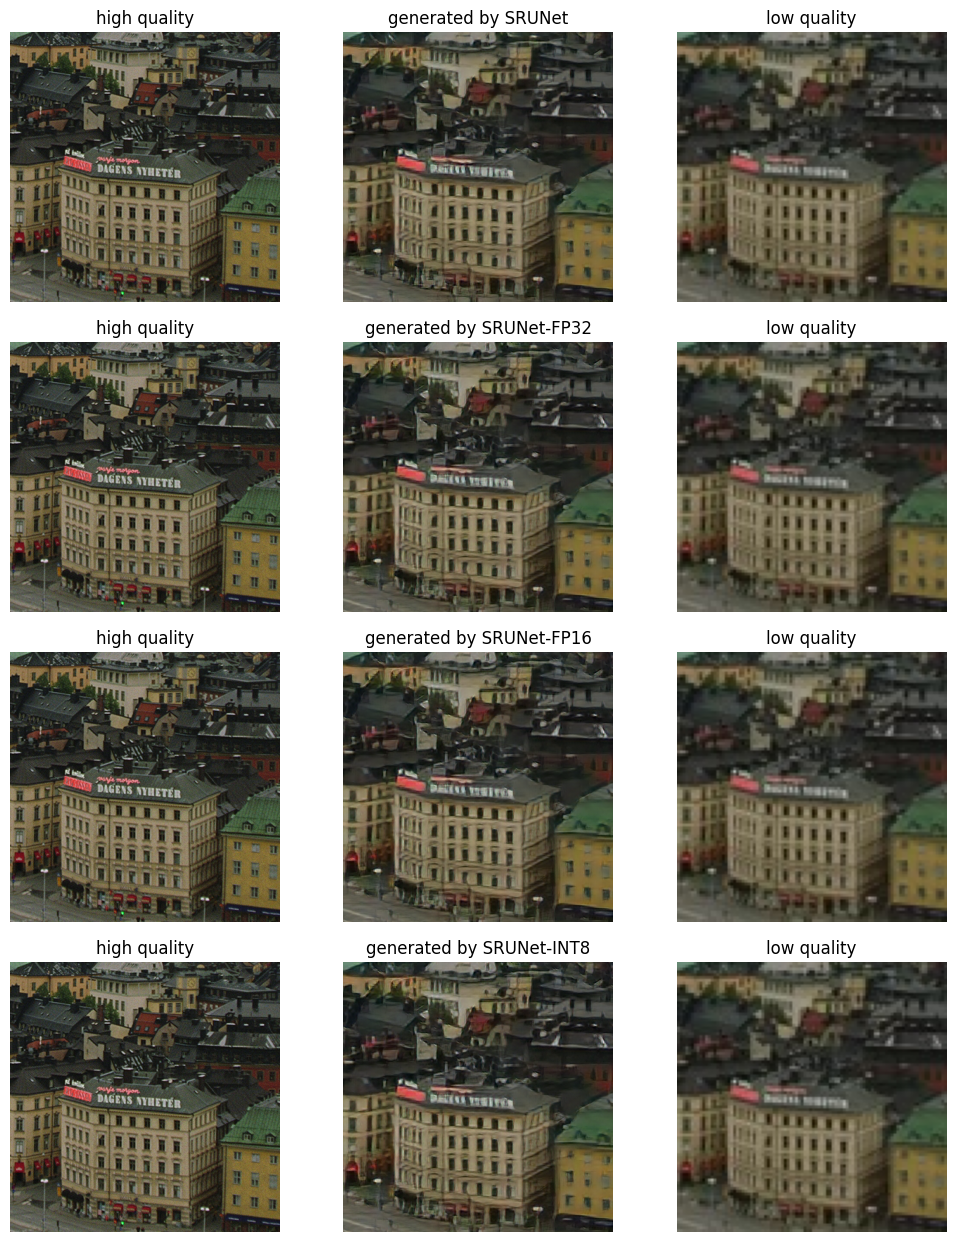
\includegraphics[width=0.8\textwidth]{static/srunet_qualitative_results.png}
\caption{Qualitative results for each variation of the SRUNet model on a test patch.}
\label{fig:qualitative-srunet}
\end{figure*}
